\documentclass[journal, a4paper]{IEEEtran}

% some very useful LaTeX packages include:

\usepackage{ctex}
\usepackage{graphicx}
\usepackage{animate}
\usepackage{subfigure}
\usepackage{url}
\usepackage{amssymb}
\usepackage{amsmath}
\usepackage{cite}
\usepackage{multirow}
\usepackage{listings}
\usepackage{booktabs}
\usepackage[colorlinks,linkcolor=blue]{hyperref}
\usepackage{listings}
\usepackage{xcolor}

\lstset{
    basicstyle=\scriptsize,
    breaklines=true,
    columns=fixed,
    frame=none,
    backgroundcolor=\color[RGB]{245,245,244},
    keywordstyle=\color[RGB]{40,40,255},
    numberstyle=\footnotesize\color{darkgray},
    commentstyle=\it\color[RGB]{0,96,96},
    stringstyle=\rmfamily\slshape\color[RGB]{128,0,0},
    showstringspaces=false,
    language=C,
    tabsize=2
}
\lstset{
    emph={chan, system, clock, broadcast, A[], and,imply},
    emphstyle={\color[RGB]{40,40,255}}%
}

\usepackage{draftwatermark}
\SetWatermarkText{ZHZ's Report}

% Your document starts here!
\begin{document}

% Define document title and author
	\title{智能会议室系统\\——形式语言与自动机课程大作业}
    \author{张煌昭$^\dagger$\thanks{$\dagger$ 学号:1901111303 邮箱:zhang\_hz@pku.edu.cn} 信息科学技术学院}
	\markboth{智能会议室系统}{}
	\maketitle

% Write abstract here
\begin{abstract}
物联网(IoT)技术目前已经逐步进入人们的生活之中,设备通过互联的方式进行自动调控,创造宜居、舒适、方便的生活和工作环境。本次大作业,我们设想了一个基于IoT应用系统的智能会议室的场景,对会议室内进行自动的调温和调光。此外,我们在UPPAAL工具上对该系统进行了建模,并对该系统进行了性质验证。该智能会议室系统通过了所有安全性和时间性质的验证。
\end{abstract}

% Main Part

\section{系统的非形式化描述}
\label{section:informal}

我们假设存在这样的一个基于IoT应用系统的智能会议室系统,其中安装有灯、电动窗帘、空调、投影仪灯设备,室内还安装有光强传感器和温度传感器用于监测室内的光强和温度,设备和传感器在控制系统的控制下对会议流程和室内环境进行控制;此外,系统支持手动模式,可以通过开关直接控制所有设备。系统需要提供的服务如下:

1) 会议系统。在开始会议时,系统首先自动关闭窗帘和灯,之后打开投影仪;会议进行的过程中,需要保证投影仪打开,并且保证投影仪和窗帘、投影仪和灯不能同时打开;会议结束后,投影仪关闭,灯和窗帘根据情况进行自动调节。

2) 温度控制。系统根据温度控制器采集到的温度信号(过冷、过热或适宜)控制空调系统(制热、制冷或关闭),温度传感器的采样间隔不大于一分钟。在接收到传感器信号后,空调的响应时间需要少于5秒。

3) 光强控制。光强控制系统只会在没有会议进行时启动,系统每分钟采样一次光强信号(强光、柔光或黑暗)。当光强过强时,窗帘自动拉上,灯自动关闭;在柔光时,可以拉开窗帘并关灯或合上窗帘并开灯,为了节能减排,规定拉开窗帘并关灯;在黑暗情况下,无需考虑窗帘直接自动开灯。在接收到传感器信号后,灯和窗帘的响应时间需要少于5秒。

4) 手动模式。手动模式下,所有自动控制系统全部关闭,用户可以通过开关来直接控制所有设备,为了保证系统安全性,在手动控制的过程中,投影仪和窗帘、投影仪和灯不能同时打开必须被保证。用户可以通过开关来切换手动模式和自动模式。

结合上述要求,可以总结出系统需要满足如下性质:

\begin{itemize}
    \item 系统内各个组件不发生死锁;
    \item 投影仪和窗帘、投影仪和灯不会同时打开;
    \item 温度传感器和光强传感器采样间隔时间小于60s;
    \item 接收到温度信号后,空调在5s内响应;
    \item 接收到光强信号后,窗帘和灯在20s内响应。
\end{itemize}

\section{系统的形式化描述}
\label{section:formal}

\begin{table}[b]\scriptsize
    \centering
    \begin{tabular}{cccccc}
    \toprule
        类型 & 实体 & 标识符 & 类型 & 实体 & 标识符 \\
    \midrule
        \multirow{4}{*}{设备} & 灯 & Lamp & \multirow{7}{*}{开关} & 灯的开关 & setLamp \\
         & 窗帘 & Curtain & & 窗帘开关 & setCurtain \\
         & 空调 & AC & & 空调遥控器 & setAC \\
         & 投影仪 & Projector & & 投影仪开关 & setProjector \\
    \cline{1-3}
        \multirow{2}{*}{控制器} & 中央控制器 & Controller & & 会议开关 & setConf \\
         & 重置器 & Reset & & 模式开关 & setAuto \\
    \cline{1-3}
        \multirow{2}{*}{传感器} & 光强传感器 & envLight & & 重置按钮 & setReset \\
         & 温度传感器 & envTemp \\
    \bottomrule
    \end{tabular}
    \caption{系统中的实体}
    \label{table:entity}
\end{table}

我们设计的智能会议室系统中的实体如表\ref{table:entity}中列出,包括IoT设备、开关和控制器三类。与第\ref{section:informal}节不同的是,我们的设计中加入了重置器,用于在模式切换时对系统状态进行重置;相应的,设计中加入了重置按钮,用于手动的对系统进行重置。

各个设备、传感器和中央控制器的部分状态在表\ref{table:state}中列出,由于UPPAAL的软件限制,在实现的过程中需要通过加入很多没有时延的Commited状态来进行同步。状态转移以及信号等将在第\ref{section:automata}节进行详细说明。

系统中的属性如表\ref{table:property}中列出,包括环境属性(光强和温度)、模式属性、开关属性(设备是否打开等)和时钟属性,各个属性的取值及相应的含义均在表\ref{table:property}中列出。

\begin{table}[t]\scriptsize
    \centering
    \begin{tabular}{ccc}
    \toprule
        实体 & 状态及含义 & 初始状态 \\
    \midrule
        Lamp & on-打开,off-关闭 & on \\
        Curtain & open-打开,close-关闭 & open \\
        Projector & on-打开,off-关闭 & off \\
        AC & off-关闭,warm-制热,cool-制冷 & off \\
    \midrule
        envLight & wait-等待,check-采样 & wait \\
        envTemp & wait-等待,check-采样 & wait \\
    \midrule
        \multirow{3}{*}{Controller} & auto-自动,dark-黑暗,subdued-柔光, & \multirow{3}{*}{auto} \\
         & strong-强光,manual-手动,high-过热, & \\
         & low-过冷, comfortable-适宜 & \\
    \bottomrule
    \end{tabular}
    \caption{系统中的各设备的状态}
    \label{table:state}
\end{table}

\begin{table}[t]\scriptsize
    \centering
    \begin{tabular}{cccc}
    \toprule
        属性 & 类型 & 标识符 & 值域及含义 \\
    \midrule
        光强 & int & envLight & 0-黑暗,1-柔光,2-强光 \\
        温度 & int & envTemperature & 0-适宜,1-过冷,2-过热 \\
        系统模式 & int & autoMode & 0-手动,1-自动 \\
        灯是否打开 & int & lampOn & 0-关闭,1-打开 \\
        窗帘是否拉开 & int & curtainOpen & 0-合上,1-拉开 \\
        空调模式 & int & acMode & 0-关闭,1-制热,2-制冷 \\
        投影仪是否打开 & int & projectorOn & 0-关闭,1-打开 \\
        会议是否开启 & int & confOn & 0-关闭,1-开启 \\
        光强传感器时钟 & clock & lightSenserClock & 光强传感器采样间隔 \\
        温度传感器时钟 & clock & tempSenserClock & 温度传感器采样间隔 \\
        调光系统时钟 & clock & lampClock & 调光系统响应时间 \\
        调温系统时钟 & clock & acClock & 调温系统响应时间 \\
    \bottomrule
    \end{tabular}
    \caption{系统中的属性}
    \label{table:property}
\end{table}

\section{系统成分及自动机建模}
\label{section:automata}

整个系统由表\ref{table:entity}中的设备、控制器、传感器、开关各一个构成,我们使用UPPAAL工具对其进行自动机建模,下面对各个部件分的自动机建模分别进行说明。

\begin{figure}[t]
    \centering
    \subfigure[Lamp]{
        \includegraphics[width=0.46\columnwidth]{images/Lamp.png}
        \label{figure:iot:subfigure:lamp}
    }
    \subfigure[Curtain]{
        \includegraphics[width=0.46\columnwidth]{images/Curtain.png}
        \label{figure:iot:subfigure:curtain}
    }
    \subfigure[AC]{
        \includegraphics[width=0.46\columnwidth]{images/AC.png}
        \label{figure:iot:subfigure:ac}
    }
    \subfigure[Projector]{
        \includegraphics[width=0.46\columnwidth]{images/Projector.png}
        \label{figure:iot:subfigure:projector}
    }
    \caption{物联网设备的自动机建模。图\ref{figure:iot:subfigure:lamp}-图\ref{figure:iot:subfigure:projector}分别对应灯、窗帘、空调和投影仪的自动机建模。}
    \label{figure:iot}
\end{figure}

图\ref{figure:iot}所示为系统中所有物联网设备的自动机建模,包括灯、窗帘、空调和投影仪。其中灯、窗帘和投影仪均具有两个稳定状态,即打开(on或open)和关闭(off或close),这些设备在接收到开启(或关闭)信号后执行开启(或关闭)动作,将自己的打开属性设置为1(或0)。以灯为例,初始状态为off,在收到打开灯的openLamp信号后,将灯的打开状态设置为1,到达on状态(由于中间的状态为Commited,不存在时延,因此可以视为同时完成);同样的,在on状态时,收到关闭灯的closeLamp信号后,将灯的打开状态设置为0,回到off状态。窗帘和投影仪同理。空调具有三个稳定状态,分别为关闭(off)、制热(warm)和制冷(cool)。与灯类似的,空调的初始状态为off,在接收到warmAC信号后把acMode设置为2开始制热并跳转为warm状态,在接收到coolAC信号后把acMode设置为1开始制冷并跳转为cool状态;同样的,在warm状态收到closeAC或coolAC信号时会关闭或制冷并跳转为off或cool状态,在cool状态收到closeAC或warmAC信号时会关闭或制热并跳转为off或warm状态。

\begin{figure}[t]
    \centering
    \subfigure[envLightSenser]{
        \includegraphics[width=0.67\columnwidth]{images/light.png}
        \label{figure:senser:subfigure:light}
    }
    \subfigure[envTemperatureSenser]{
        \includegraphics[width=0.67\columnwidth]{images/temperature.png}
        \label{figure:senser:subfigure:temperature}
    }
    \caption{传感器的自动机建模。图\ref{figure:senser:subfigure:light}和图\ref{figure:senser:subfigure:temperature}分别光强传感器和温度传感器的自动机建模。}
    \label{figure:senser}
\end{figure}

\begin{figure*}[t]
    \centering
    \subfigure[setReset]{
        \includegraphics[width=0.15\columnwidth]{images/setReset.png}
        \label{figure:switch:subfigure:setReset}
    }
    \subfigure[setAuto]{
        \includegraphics[width=0.25\columnwidth]{images/setAuto.png}
        \label{figure:switch:subfigure:setAuto}
    }
    \subfigure[setConference]{
        \includegraphics[width=0.25\columnwidth]{images/setConference.png}
        \label{figure:switch:subfigure:setConference}
    }
    \subfigure[setCurtain]{
        \includegraphics[width=0.25\columnwidth]{images/setCurtain.png}
        \label{figure:switch:subfigure:setCurtain}
    }
    \subfigure[setLamp]{
        \includegraphics[width=0.25\columnwidth]{images/setLamp.png}
        \label{figure:switch:subfigure:setLamp}
    }
    \subfigure[setProjector]{
        \includegraphics[width=0.25\columnwidth]{images/setProjector.png}
        \label{figure:switch:subfigure:setProjector}
    }
    \subfigure[setAC]{
        \includegraphics[width=0.25\columnwidth]{images/setAC.png}
        \label{figure:switch:subfigure:setAC}
    }
    \caption{开关的自动机建模。图\ref{figure:switch:subfigure:setReset}和图\ref{figure:switch:subfigure:setAC}分别对应重置按钮、模式开关、会议开关、窗帘开关、灯开关、投影仪开关和空调遥控器的自动机建模。}
    \label{figure:switch}
\end{figure*}

图\ref{figure:senser}所示为系统中的传感器的自动机建模,包括光强传感器和温度传感器。其中光强传感器的初始状态为wait,跳转时设置光强等级,并发出相应的光强信号,转移至check状态;在check状态停留一段时间(小于60s)后,重置时钟并返回至wait状态。温度传感器同理。

图\ref{figure:switch}所示为系统中的开关的自动机建模,包括重置按钮、模式开关、会议开关、窗帘开关、灯开关、投影仪开关和空调遥控器。所有开关都只有一个稳定状态wait,通过从wait状态跳转到Commited状态再回到wait状态,开关可以发出相应的开关信号(或模式切换信号),该信号被设备或中央控制器接收,执行对应的动作。模式开关和会议开关在切换的同时,还需要分别设置模式属性(autoMode)和会议开始属性(confOn)。重置按钮可以在wait状态,通过回路跳转发出doreset重置信号,使得整个系统重置到初始状态。

\begin{figure}
    \centering
    \includegraphics[width=0.7\columnwidth]{images/reset.png}
    \caption{重置器的自动机建模。}
    \label{figure:reset}
\end{figure}

图\ref{figure:reset}所示为系统中的重置器的自动机建模,由于在系统切换时需要对系统中的设备进行状态重置,以及允许用户通过重置按钮来直接重置系统,必须在系统中引入这一模块。重置器分别发送closeLamp、closeProjector和closeAC信号来关闭灯、投影仪和空调,并与此同时直接将灯(lampOn)、投影仪(projectorOn)和空调(acMode)的开关状态置零关闭;之后重置器发送openCurtain信号并将curtainOpen置1来打开窗帘;最后将confOn置0以关闭会议,到达done状态,完成系统重置。

图\ref{figure:controller}所示为系统中的中央控制器的自动机建模,该模块可以分作手动模式、自动模式和切换模式三个子模块,三个子模块分别在图\ref{figure:controller}中用蓝色虚线、红色点横线和黄色点线框出。

手动模式(蓝色虚线框)下,控制器只有manual一个稳定状态,并在manual状态等待开关被拨动传来的信号。控制器收到重置按钮发出的doreset信号后,发出reset信号对系统进行重置。控制器收到空调遥控器发出的acwarm、accool和acoff信号后,分别发出warmAC、coolAC和closeAC信号给空调,最后回到manual状态。由于有投影仪和灯、投影仪和窗帘不能同时打开的限制,打开这三个设备时需要关闭不能共存的设备。例如,当控制器收到投影仪开关发来的openProjector信号后,必须先发出closeCurtain和closeLamp信号,再发出openProjector信号。当控制器收到灯、窗帘和投影仪开关发出的关闭信号后,直接发出关闭信号来关闭对应的设备即可。

\begin{figure*}
    \centering
    \includegraphics[width=1.7\columnwidth]{images/Controller.png}
    \caption{中央控制器的自动机建模。与manual状态相连的回路(蓝色虚线框出)对应手动模式下的控制逻辑,与auto状态相连的回路(红色点横线框出)对应自动模式下的控制逻辑,manual状态与auto状态相连的部分(黄色点线框出)对应模式切换的控制逻辑。}
    \label{figure:controller}
\end{figure*}

自动模式(红色点横线框)下,控制器一般停留在auto状态等待信号。当控制器收到会议开关发来的开始会议的conf信号后,发出closeLamp和closeCurtain信号关闭灯和窗帘,之后发出openProjector信号打开投影仪开始会议;当控制器收到会议结束的noconf信号后,直接发出closeProjector信号关闭投影仪,灯和窗帘会通过自动调光逻辑进行调整。
auto状态右下方的三个回路从左到右分别为黑暗、柔光和强光下自动调光的控制逻辑:黑暗时,若正在进行会议则说明投影仪打开、则不进行开灯操作,否则发出openLamp信号开灯;柔光时,首先发出closeLamp信号关灯,之后根据是否正在进行会议来决定是否发出openCurtain信号打开窗帘;强光时,直接发出closeLamp和closeCurtain信号关灯和合上窗帘。
auto状态左下方的三个回路从左到右分别为过热、过冷和适宜气温下自动调温的控制逻辑:过热时,发出coolAC信号启动空调制冷;过冷时,发出warmAC信号启动空调制热;温度适宜时,发出closeAC信号关闭空调。

模式切换(黄色点线框)时,需要发出reset信号对整个系统进行重置,否则会使得投影仪与灯、投影仪与窗帘不同时打开的安全性约束出错。

\section{系统定义}
\label{section:system}

整个系统包含第\ref{section:automata}节中定义的自动机各一个,其代码如下所示。

\lstset{numbers=right}
\begin{lstlisting}
_Lamp = Lamp();
_Curtain = Curtain();
_Projector = Projector();
_AC = AC();
_Controller = Controller();
_envLightSenser = envLightSenser();
_envTemperatureSenser = envTemperatureSenser();
_setConference = setConference();
_setAuto = setAuto();
_setLamp = setLamp();
_setAC = setAC();
_setCurtain = setCurtain();
_setProjector = setProjector();
_reset = Reset();
_setReset = setReset();
system _Lamp, _Curtain, _Projector, _AC, _Controller,
    _envLightSenser, _envTemperatureSenser, _setConference,
    _setAuto, _setLamp, _setAC, _setCurtain, _setProjector,
    _reset, _setReset;
\end{lstlisting}

系统中的实体属性定义如下,其分别与表\ref{table:property}对应。

\lstset{numbers=left}
\begin{lstlisting}
int envLight = 0, envTemperature = 0;
int confOn = 0, lampOn = 0,
int projectorOn = 0, curtainOpen = 0, acMode = 0;
clock lampClock, acClock;
clock lightSenserClock, temperatureSenserClock;
int autoMode = 1;
\end{lstlisting}

系统中进行通信的信号定义如下。其中第1行为室内光强和温度的信号,第2-5行为中央控制器控制各个设备及重置器的信号,第6-8行为各个开关被拨动时发送给中央控制器的信号。

\lstset{numbers=left}
\begin{lstlisting}
chan EnvLight[3], EnvTemperature[3];
chan conf, noconf
broadcast chan warmAC, coolAC, closeAC, openLamp, closeLamp;
broadcast chan openCurtain, closeCurtain;
broadcast chan openProjector, closeProjector, reset;
chan toAuto, toManual,lampon, lampoff,acwarm, accool, acoff;
chan curtainopen, curtainclose,projectoropen, projectorclose;
chan doreset;
\end{lstlisting}

对系统进行模拟。在模拟光强变化时,系统的通信如图\ref{figure:run1}所示,符合预期,所有自动调光逻辑运行正常;在模拟温度变化时,系统的通信如图\ref{figure:run2}所示,同样符合预期,所有自动调温逻辑运行正常;在模拟手动模式时,系统的通信如图\ref{figure:run3}所示,也符合预期,模式切换、手动开关及重置按钮的逻辑正常。

\section{系统性质}
\label{section:property}

根据第\ref{section:informal}中定义的约束,可以逐条在UPPAAL的验证其上写出如下性质验证。

\lstset{numbers=left}
\begin{lstlisting}
A[] _Projector.on+ _Curtain.open < 2
A[] _Projector.on + _Lamp.on < 2
A[] _envTemperatureSenser.check imply temperatureSenserClock <= 60
A[] _envLightSenser.check imply lightSenserClock <= 60
A[] _Lamp.on imply lampClock<=20
A[] _Lamp.off imply lampClock<=20
A[] _Curtain.open imply lampClock<=20
A[] _Curtain.close imply lampClock<=20
A[] _AC.cool imply acClock<=5
A[] _AC.warm imply acClock<=5
A[] _AC.off imply acClock<=5
A[] _reset.done imply confOn==0 and lampOn==0 and projectorOn==0 and curtainOpen==1 and acMode==0
A[] not deadlock
\end{lstlisting}

其中第1-2行要求投影仪和窗帘、投影仪和灯不会同时打开,第3-4行要求光强和温度传感器采样间隔不大于60s,第5-8行要求自动调光的反应时间不大于20s,第9-11行要求自动调温的反应时间不大于5s,第12行要求重置器能够对系统进行初始化,第13行要求系统不发生死锁。

对以上性质逐条进行验证,结果如图\ref{figure:property}所示,所有性质均通过了性质验证。

\begin{figure}[t]
    \centering
    \includegraphics[width=\columnwidth]{images/property.png}
    \caption{性质验证结果。所有性质均通过验证。}
    \label{figure:property}
\end{figure}

\section{感想与建议}
\label{section:suggestion}

一个系统从构思到成功进行系统建模并通过性质验证,并没有想象中的那么容易。在人类脑海中很简单的过程,在变迁系统中可能需要十几乃至几十个状态才能很好地表示。在何处进行时间性质的控制、如何处理每个状态的所有条件跳转、如何通过合并尽可能简化系统, 都是需要额外费脑筋的事情。

建议之后布置使用UPPAAL的大作业时,附上经过挑选的软件教程或者tutorial。因为网上论坛里鲜有关于该软件的入门教程和问答,本次作业前期搜集Uppaal的使用方式花了不少时间,效果也一般,需要同学间互帮互助,才勉强能用起软件的基本功能。许多功能都是在\cite{behrmann2004tutorial}和\cite{david2011uppaal}两份英文教程中发现的,而这些功能却恰好能够大大提升建模效率。

\bibliography{ref}
\bibliographystyle{plain}

\clearpage
\onecolumn

\begin{figure}
    \centering
    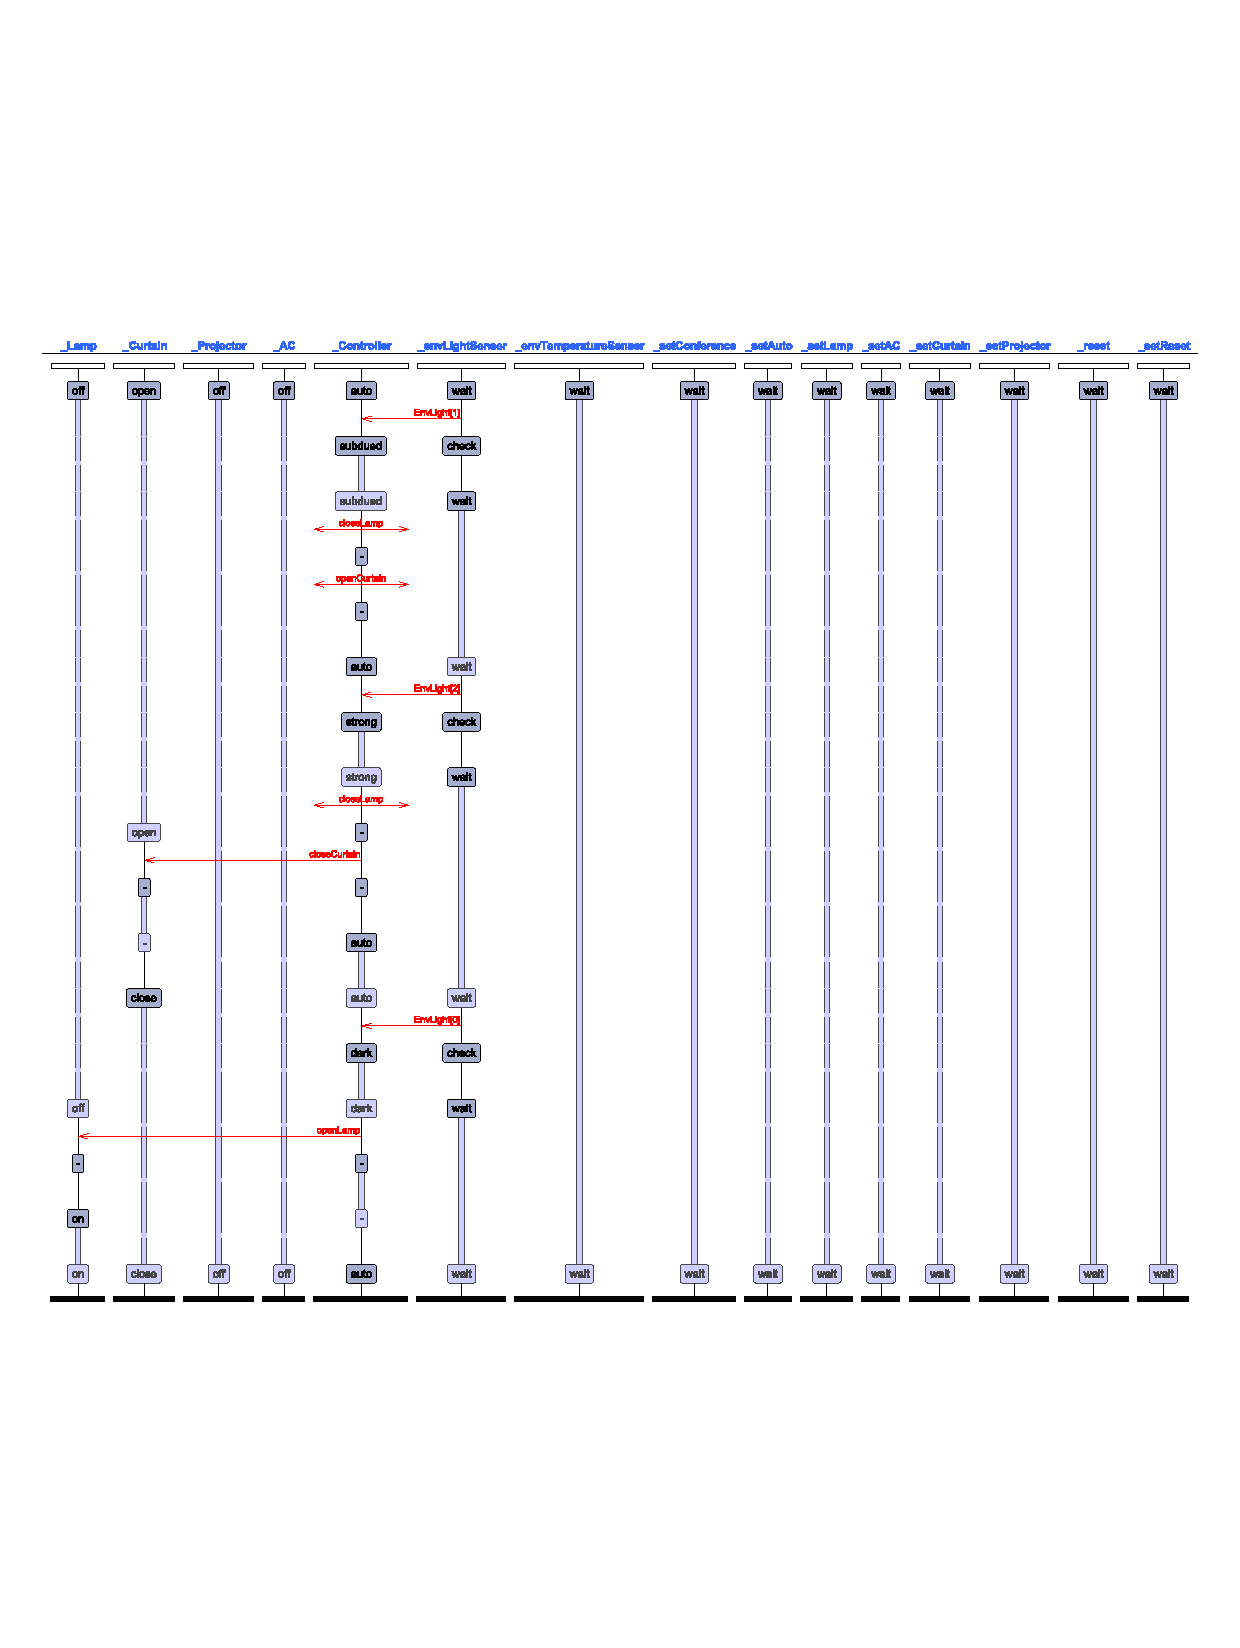
\includegraphics[width=\columnwidth]{images/run1.pdf}
    \caption{系统在光强变化下的通信情况的trace。}
    \label{figure:run1}
\end{figure}

\begin{figure}
    \centering
    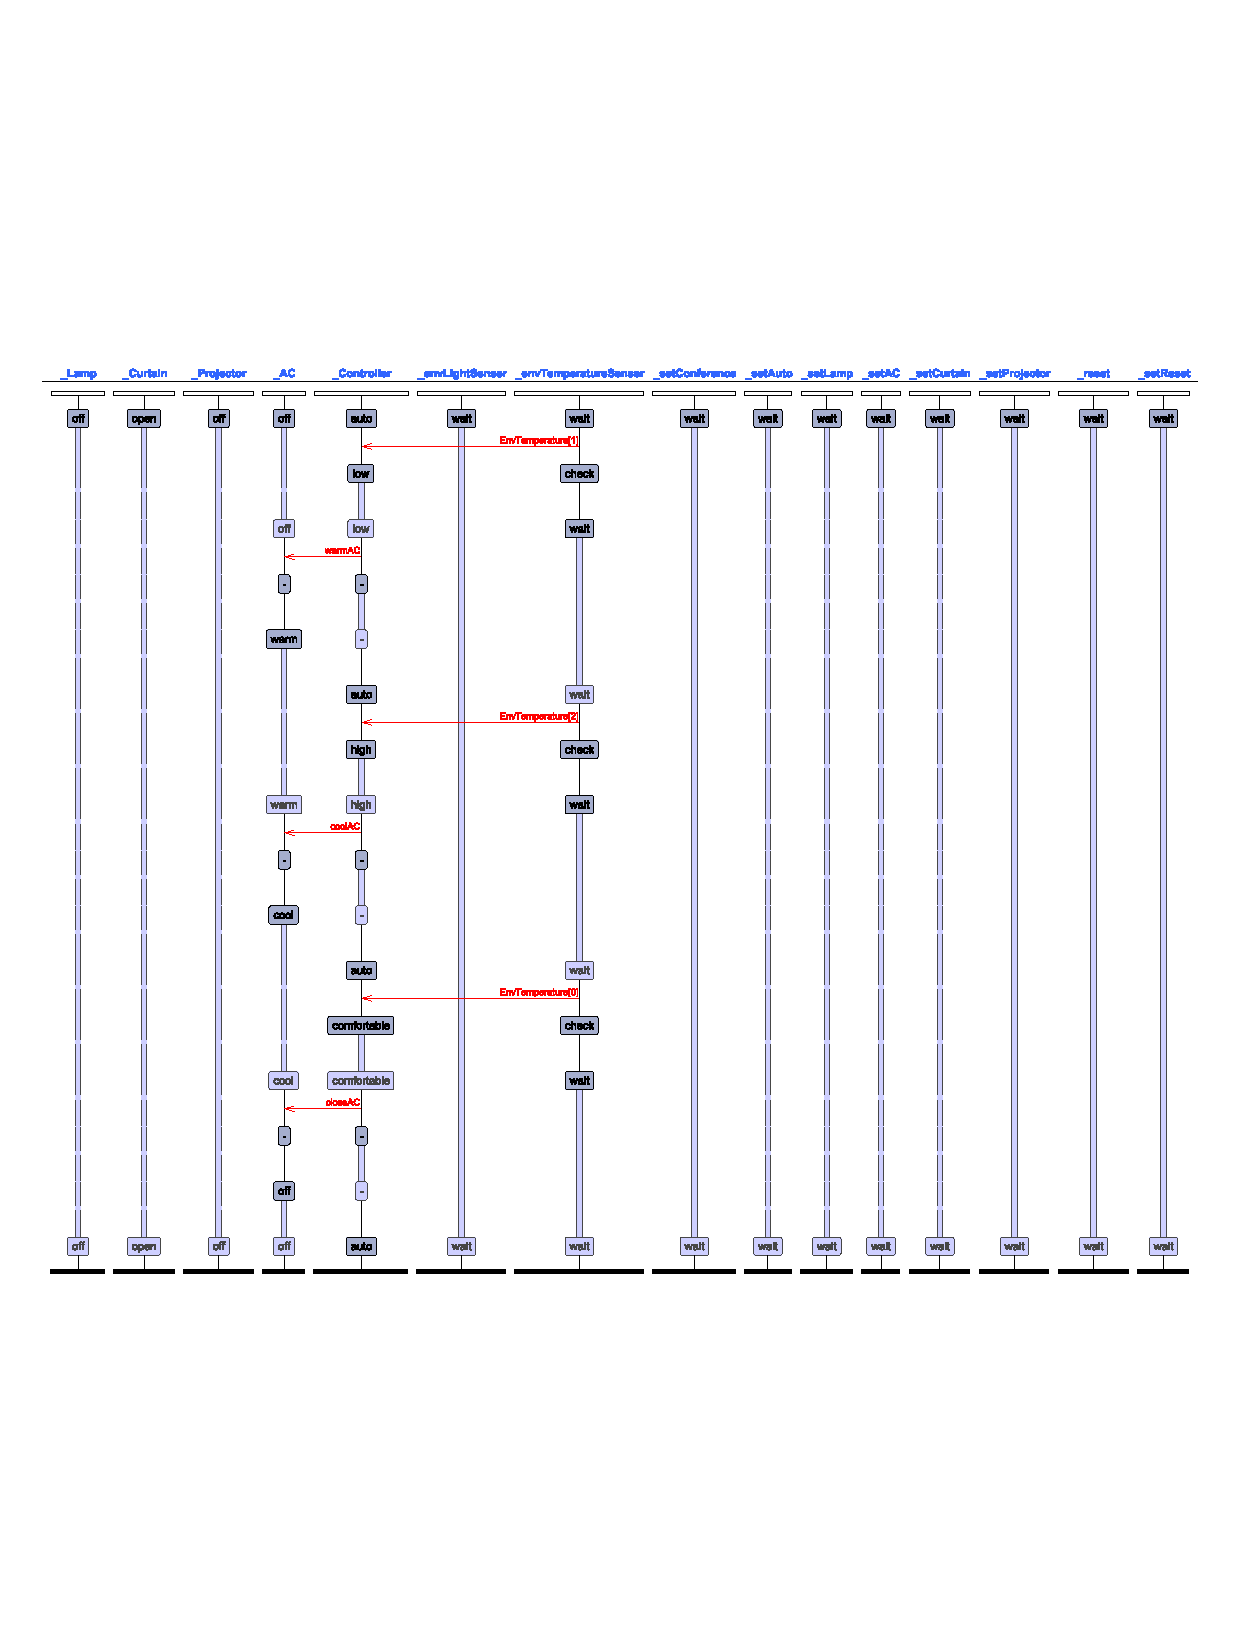
\includegraphics[width=\columnwidth]{images/run2.pdf}
    \caption{系统在温度下的通信情况的trace。}
    \label{figure:run2}
\end{figure}

\begin{figure}
    \centering
    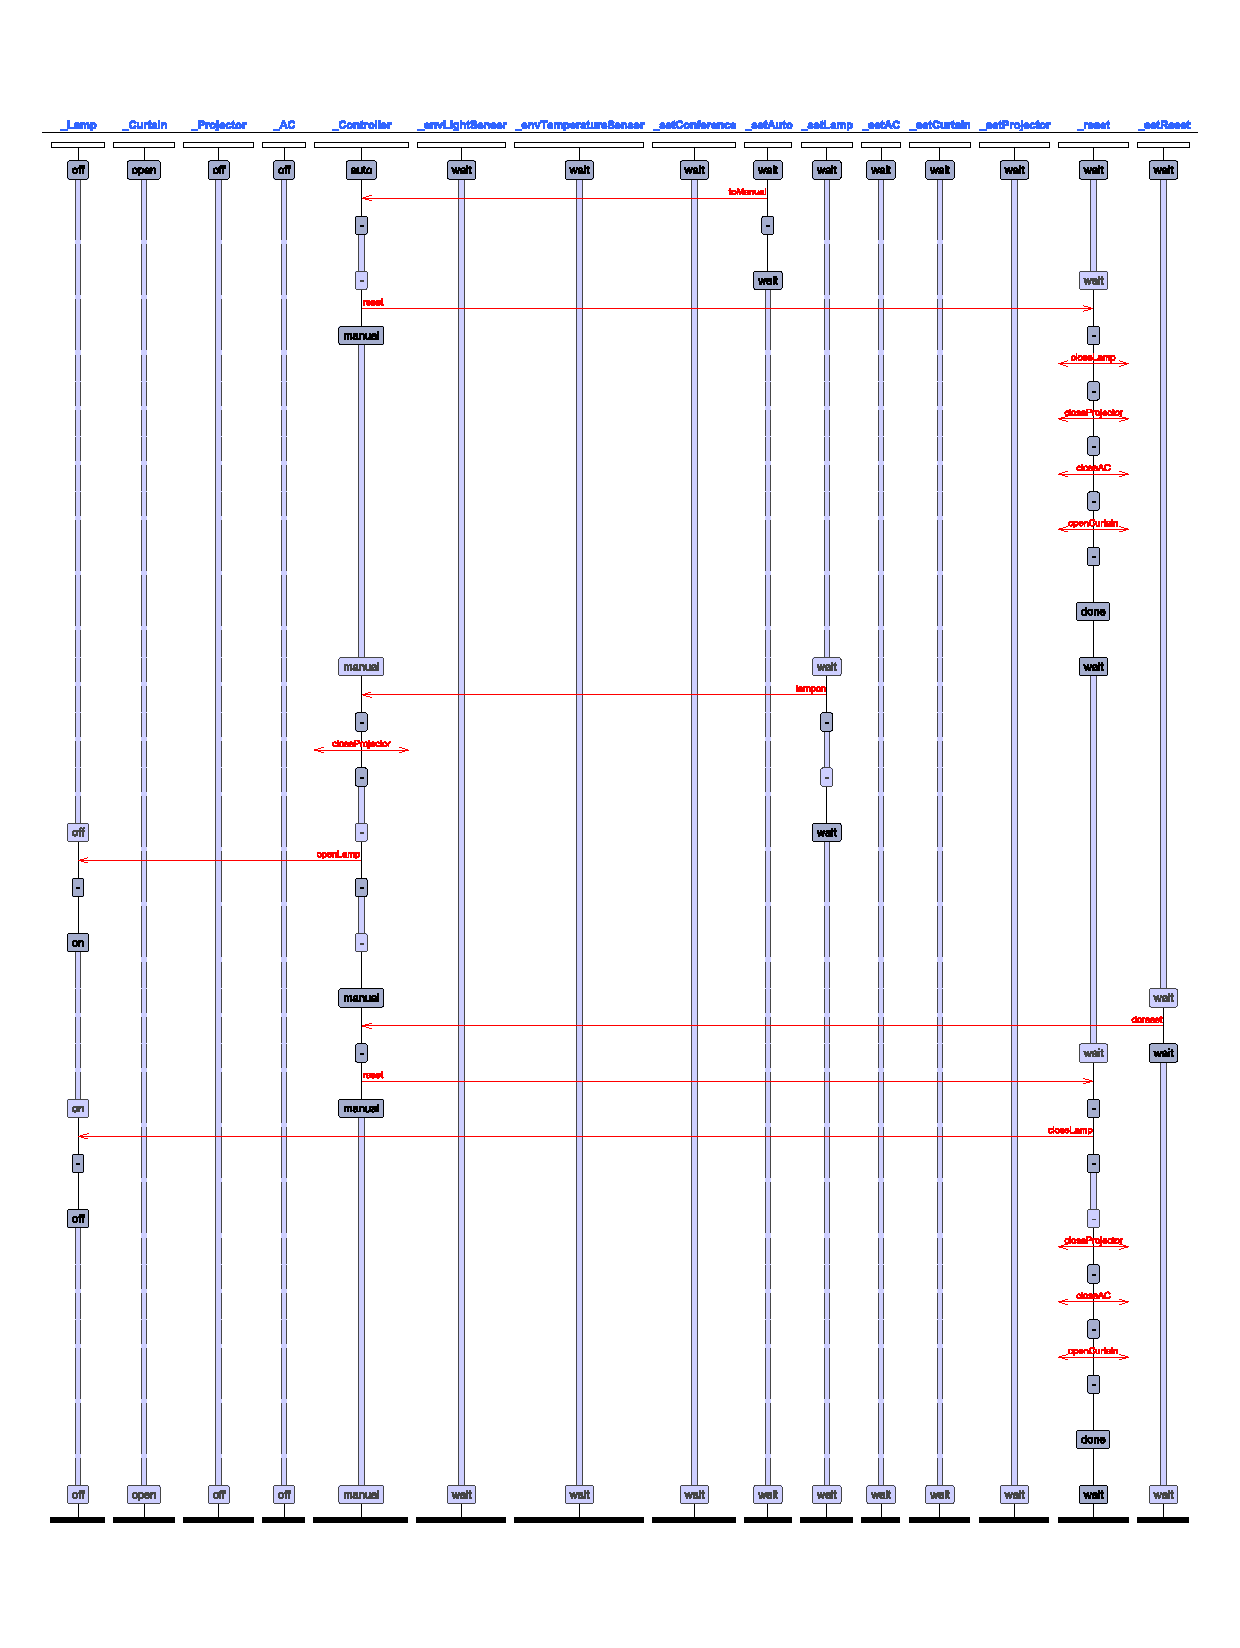
\includegraphics[width=\columnwidth]{images/run3.pdf}
    \caption{系统在手动模式下下的通信情况trace。}
    \label{figure:run3}
\end{figure}

% Your document ends here!
\end{document}